
\chapter{Background}

This chapter will give the background needed to understand the core work of this thesis. 
\section{Interactive Theorem Proving} 
\section{Lean4 Foundations} 
Lean is an interactive theorem prover and functional programming language initiated by Leonardo de Moura at Microsoft Research in 2013. Lean aims to "bridge the gap between interactive and automated theorem proving," enabling users to construct complex proofs using human insights while leveraging powerful automation features to simplify the proof process.
Lean 4 is the newest version of the Lean theorem prover, distinguished by being implemented within Lean itself. Unlike traditional theorem provers such as Coq or Isabelle, Lean provides robust metaprogramming capabilities, allowing users to extend the system using the Lean language itself.

A key feature of Lean is its unified approach to software development and verification. Users can write programs and prove properties about them using the same language, enabling direct verification of software implementations. In Lean, types, terms, and proofs are integrated within a single framework.

In the Lean system, types are first-class citizens, and there is no fundamental distinction between terms and types—types themselves are treated as terms. A term in Lean is an expression that has a specific type, and can include variables, constants, functions, or more complex constructions that follow the rules of Lean's type system. [TO DO ASK ALEX]

This integration of types as terms and propositions as programs exemplifies the Curry-Howard Correspondence, a fundamental principle connecting logic and computation. According to this correspondence, propositions can be represented as types, and proofs as programs of those types.



There are two modes to construct proofs in Lean. The term mode, the directly proofs a statement by providing a term of the corresponding type. The user explicitly constructs an inhabitant (a value) of the type representing the proposition to be proven. Tactic mode is a mode where proofs are constrcuted step-by-step and make use of tactics, which are introdcued bellow, to transform proof goals. 

To construct proofs in Lean, users can employ two complementary approaches. In term mode a user can directly provide a term of the corresponding type that proves the proposition. In this approach, the user explicitly constructs an inhabitant (a value) of the type representing the proposition to be proven. In tactic mode, commands, so called tactics are used to transform the proof goal and step-by-step develop a proof. Tactics will be introduced in detail in a subsection. 


\textbf{Bit Vectors in Lean:}
Bitvectors are fixed-width binary sequences that provide a mathematical abstraction for modeling machine-level data representation. A bitvector of width $w$ formally represents an element from the set $\{0, 1, \ldots, 2^w - 1\}$, which corresponds to the possible values that can be stored in a $w$-bit register. This representation is foundational in formal verification of hardware designs, instruction set architectures, and low-level software systems like compilers where bit vectors e.g enable reasoning about register operations. The Lean theorem prover supports reasoning about finite bit vectors through the \textit{BitVec} type, which represents a natural number \textit{n} with a proof that \( n < 2^w \). Specifcally \textit{BitVec} is implemented as "a wrapper around \textit{Fin} with a suitable bound". In Lean, the type \textit{Fin n} represents the finite set of natural numbers strictly less than n. An element of type \textit{Fin n} consist of a natural number \textit{val}, and a proof that \textit{val \( < \) n}. Both \textit{Fin} and  \textit{BitVec} exemplify Lean's dependent typing capabilities, as their type definitions depend on a value (the upper bound n or width w, respectively). \textit{Fin} itself is built upon \textit{Nat} (natural numbers), which have strong support in Lean's kernel.\newline


\begin{lstlisting} [language=Python, caption= bit vector represenation in Lean]
structure Fin (n : Nat) where
  val : Nat
  isLt : val < n 
-- type Fin n represents the finite set of natural numbers
strictly less than n, including a proof that val < n.

def BitVec (w : Nat) := { n : Nat // n < 2^w }
-- type BitVec represents the finite set of natural numbers
val, including a proof that n < 2^w.
\end{lstlisting}

 The design choice of wrapping the implementation of \textit{BitVec} around \textit{Fin} and \textit{Nat} allows for efficient reasoning about bit vectors by leveraging Lean's optimized natural number operations while maintaining the formal constraint of boundedness through dependent typing.
In compiled code, the representations of \textit{Fin, BitVec}  and \textit{Nat} are indistinguishable and efficient, leaving only the underlying natural number representation.



\begin{lstlisting} [language=Lean, caption= Example of defining a Fin in the range of 0 to 31 with value 19 in Lean]
def exampleFin : Fin 32  :=  <19 , by simp [Nat.reduceLT]>
\end{lstlisting}
\begin{lstlisting} [language=Lean, caption= Example of defining a BitVec of width 32 with value 42 in Lean]
def bv32_ex1 : BitVec 32 :=  
            <42, by simp [Nat.reducePow, Nat.reduceLT]>
def bv32_ex2 : BitVec 32 :=  42#32
def bv32_ex3 : BitVec 32 :=  BitVec.ofNat 32 43 
\end{lstlisting}
 Lean provides multiple approaches for creating values of type \txtit{w} (Listing 2.3) . Whether a bit vector is interpreted as signed or unsigned depends on the bit vector operation used. Lean provides a comprehensive set of operations for both interpretations.
TO DO: move the text above the example 

\textbf{Automated Reasoning with bv\_decide:}
To support automated reasoning about fixed-width bit vectors, Lean provides the \textit{bv\_decide} tactic. \textit{Bv\_decide}, a current research effort by the University of Cambridge, is a fully Lean 4-integrated tactic for solving fixed-width bit vector problems. The tactic targets proof goals involving fixed-width bit vector operations and booleans and automates proof goal resolution by combining various existing algorithms and techniques in theorem proving and automated reasoning (figure 2.1).

TO DO : REMOVE THIS WHLE PARAGRAPH BELLOW AN DIRECTLY SKIP TO THE INTERNALS 

The bv\_decide tactic operates by processing the proof goal on multiple levels by combining internal processing with external  SMT solver integration. First, it applies standart Lean tactics to simplify and normalize the original proof goal. Then, it formulates a contradiction proof goal that is logically equivalent to the negation of the original goal. Next, the contradiction goal is bit blasted. Bitblasting is a process that decomposes bit vector operations into equivalent boolean operations. Then the bit-blasted goal is submitted to an external SMT solver. When the solver returns an UNSAT result, indicating the contradiction goal is unsatisfiable, the UNSAT certificate is reflected back into Lean's proof system. This certificate serves as evidence that the contradiction goal is false, which by logical equivalence confirms the truth of the original goal.

 The form of verification by reflecting external computation into a formal proof, is called \textit{proof by reflection}. In \textit{proof by reflection}, the result of a computation is integrated into a formal proof and seen as certificate for a proof. This in turn extends the trusted code base to the code generator that is invoked to compile and run the program that defines the computation.
\begin{figure}[htbp]
  \centering
  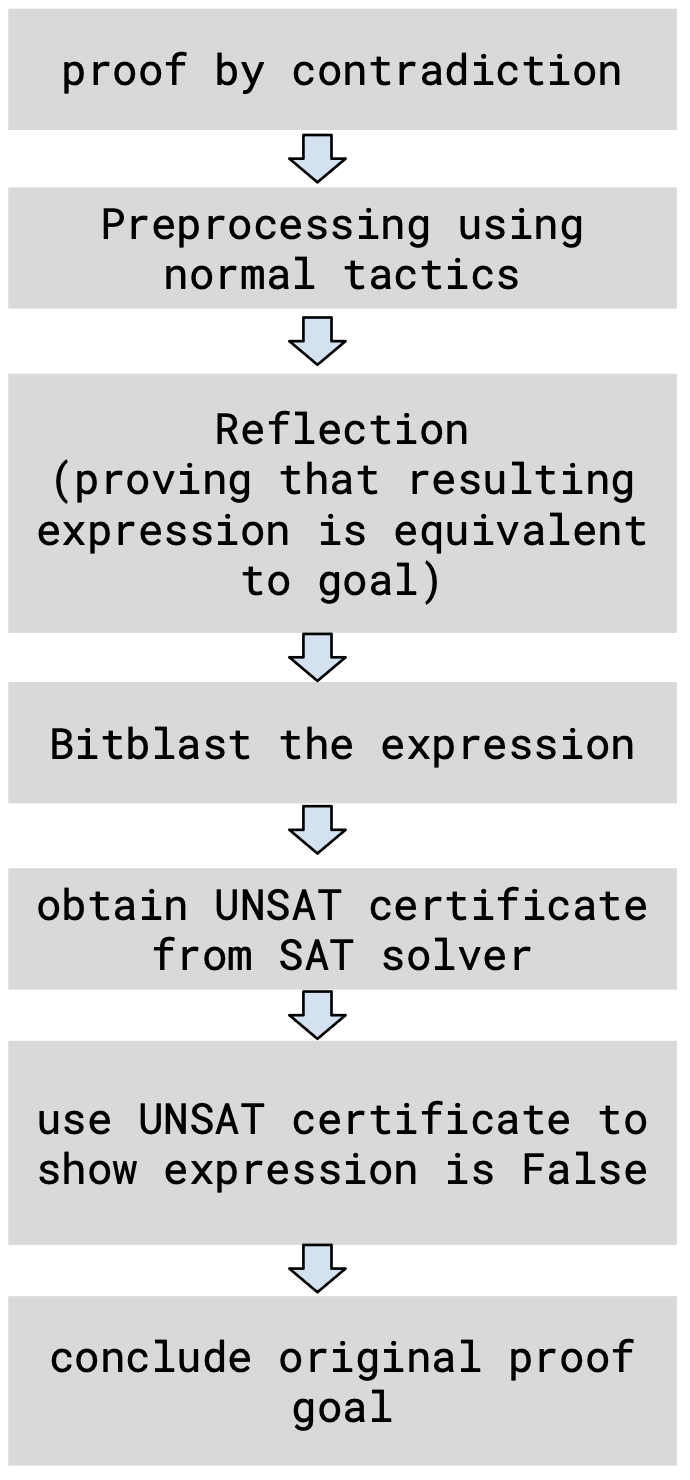
\includegraphics[scale=0.37]{thesis/bv_decide.png}
 
  \caption{Bv\_decide procedure flow}
  \label{fig:your-label}
\end{figure}

\textit{Contradiction Derivation}: Bv\_decide transforms the original goal into a contradiction form and starts a proof by contradiction. This allows for proving unsatisfiability of the contrary proof goal instead of forwards proving the original proof goal. 

\textit{Preprocessing}: Then bv\_decide normalizes and simplifies the goal by rewriting bit-vector expressions. It leverages rewrite rules inspired by the Bitwuzla SMT solver to perform these simplifications. Additionally, it performs and-flattening, which examines all currently available hypotheses, splits any conjunctions into individual hypotheses, and repeatedly applies rewriting across hypotheses until a fixed point is reached.

\textit{Reflection}: Proof by reflection is then used to show that transforming a bit-vector goal into a form where bit-vector operations are reified using additional Lean data structures preserves semantic equivalence. Wrapping bit-vector operations in these constructs enables easier processing in subsequent steps. The reflection proof guarantees that any proposition involving the enriched Lean representation is logically equivalent to a corresponding proposition about bit-vectors alone.

\textit{Bitblasting}: A verified bitblasting algorithm is then used to convert the reified bit-vector expression into an And-Inverter Graph (AIG), a data structure commonly used to efficiently represent Boolean circuits. This transformation reduces the high-level bit-vector goal to a low-level Boolean SAT problem. Finally, the AIG is translated into a conjunctive normal form (CNF) formula.

\textit{External Solving}: The CNF formula is sent to an external SMT solver, which attempts to produce an UNSAT certificate demonstrating that the formula is unsatisfiable. If the formula is satisfiable instead, the solver returns a counterexample.

\textit{Certificate Reflection}: If the SMT solver proves the formula is unsatisfiable (UNSAT), it returns an UNSAT certificate, which is imported back into Lean. The certificate is then checked within Lean ensuring that the unsatisfiability result is trustworthy and fully formalized.

\textit{Proof Construction}: Finally, the verified UNSAT certificate is used to construct a formal Lean proof of the original goal. Since the conjunction of the assumptions and the negation of the goal has been shown to be unsatisfiable, it logically follows that the original goal must be true. All previous proof steps are composed to conclude the overall proof.

Invoking the whole bv\_decide procedure to solve bit vector proof goals in Lean is illustrated below.

TO DO : want to add a more complex example regarding bv\_decide here because is way more powerful than this.
\begin{lstlisting} [language=python, caption= Discharging bit vector proof goal using bv\_decide]
theorem bv_add_comm {w : Nat} (a b : BitVec w) : 
BitVec.add a b 
    = BitVec.add b a := by
  bv_decide

theorem bv_mul_distr {w : Nat} (a b c : BitVec w) : 
  BitVec.mul a (BitVec.add b c) 
    = BitVec.add (BitVec.mul a b) (BitVec.mul a c) := by
  bv_decide
\end{lstlisting}

At the time of this thesis, bv\_decide handles a significant fragment of bit-vector logic and operations on bit vectors. However, it exhibits limitations in expressions that involve conversions between natural numbers and bit vectors, as natural numbers are unbounded in Lean and bit blasting requires a fixed-bounded width. Bv\_decide treats unknown variables or nonfixed-width bit vectors as undefined variables, however, yet attempts to resolve the goal within this abstraction. If the tactic fails to produce a proof, it returns a counterexample indicating which terms were treated as variables, providing insights into why the proof attempt failed(Listing 2.5). This interactive feedback exemplifies Lean's strength as an interactive theorem prover that leverages human-computer interaction to prove complex goals. This approach contrasts with common SMT solvers, which are proficient in solving fixed-width bit vector problems but do not support tools for interaction with the developer.


\begin{lstlisting} [language=python, caption= Example feedback by bv\_decide when trying to proof arbitrary-width bit vector theorem]
The prover found a potentially spurious counterexample:
- It abstracted the following unsupported expressions
as opaque variables: -- here the abstracted variables
will be listed.}
\end{lstlisting}





To enhance the performance of the bv\_decide procedure and avoid redundant calls to the external SMT solver, bv\_decide employs a caching mechanism for previously verified results. Additionally, the bv\_decide tactic has several configuration options to adapt its behavior to the specific structure of the proof goal e.g time-bound parameter that limits the solver execution. 
 TO DO : rethink the need to know vs the have to know ! 
Invoking bv\_normalize instead of bv\_decide runs only the normalization step of bv\_decide  and is used in proof goals where automated algebraic normalization and simplification of bit vector terms without invoking the SAT solver suffices. If the proof goal is solved by bv\_normalize the SMT solver invocation and bit-blasting are skipped by bv\_decide. 
\section{Instruction Selection and Peephole Optimizations } 

\subsection{Instruction Selection} 

During the compilation process a source programs traverse multiple transformation layers before it reaches its executable form. Code generation is a stage in a compiler backend, where the machine code for the source program is generated. Instruction selection is located at this stage in a compiler and preceeds the actual instruction scheduling and register allocation. Instruction selection is responsible for translating high-level IR instructions into concrete instructions defined by the target architecture's Instruction Set Architecture (ISA) or a lower-level IR, depending on the compiler design. This translation is non-trivial, as a single IR instruction may correspond to multiple possible sequences of machine instructions each offering different trade-offs in terms of performance, code size, or resource usage.

The IR often includes abstract operations that do not map one-to-one to the instructions available in the ISA. In many cases, the ISA supports a narrower set of operations compared to those represented in the IR e.g RISC-V does not supported a \textit{neg }instruction while LLVM IR does. Therefore, instruction selection must decompose complex IR operations into semantically equivalent sequences of machine instructions while preserving the original program behavior.
Instruction selection is critical,as it contributes to how the high-level program semantics are preserved in the final executable. If the mapping from IR instructin to machine code instruction is incorrect or not semantically faithful, the resulting executable will fail to correctly implement the source program. 

\begin{lstlisting} [language=python, caption= Example instruction selection in LLVM]
}
def ADD  : ALU_rr<0b0000000, 0b000, "add">;
def SUB  : ALU_rr<0b0100000, 0b000, "sub">;

\end{lstlisting}
In modern compiler frameworks such as LLVM, instruction selectors are typically implemented using pattern matching mechanisms. Instruction selectors rely on a set of predefined rules that match specific IR instruction patterns and replace them with the corresponding target machine instructions, when that pattern is found in the program.

The instruction selection process can also be formulated as a graph covering problem. In the graph-based approach, the IR is transformed into a graph representation, where instruction selection involves covering this graph with tiles that represent machine instructions. The goal is to find a covering that minimizes a defined cost metric e.g such as execution time or instruction count. 
Depending on the complexity of instruction selection, the compiler may produce suboptimal code. Due to the lowering process from one language to another inefficiencies can be introduced or new optimization opportunities arise due to the structure of the target-specific machine code. As a result, compilers often include peephole optimization passes after instruction selection. Peephole optimizations are introduced in detail in the next subsection.

\subsection{Peephole Optimization} 
 Peephole optimization is a fundamental technique employed in modern compilers such as GCC (a C compiler) and LLVM (low-level virtual machine). It involves analyzing short sequences of instructions and transforming them into semantically equivalent but more efficient sequences.  Peephole rewrites focus on a small, localized section of the code ("a peephole") at any one time and transform few instructions into equivalent but optimized instruction sequences.  Common types of peephole optimization include constant folding (replacing calculations on constants with their result) and strength reduction (replacing expensive operations with cheaper ones). Peephole optimizations focus on a small scope locally, but when applied throughout a program, they can significantly improve performance and reduce code size. The InstCombine pass in the LLVM compiler infrastructure is an example of a peephole optimization pass that rewrites on the IR level and performs peephole optimizations for LLVM IR.
 \begin{lstlisting}[language=Python, caption=unoptimized IR instruction sequence]
    %v1 = llvm.and %X, %Y
    %v2 = llvm.or %X, %Y
    %v3 = llvm.add %v1, %v2
\end{lstlisting}
 \begin{lstlisting}[language=Python, caption= peephole optimized IR instruction sequence ]
 %v3 = llvm.add %X, %Y
\end{lstlisting}
 [TO DO INASERT GRAPHIC OF PEEPHOLE OPTIMIZATION PASS ]
 Traditionally, peephole optimization is implemented using pattern-based rewriting. The compiler matches a predefined find pattern — which specifies a particular instruction sequence — and replaces it with a corresponding replace - pattern that yields a more optimal but meaning-preserving sequence. These rewrites can be applied at various stages of the compilation pipeline, such as on the intermediate representation level to improve the IR after high-level transformations or at the assembly level to refine the final machine code. In this work, we will implement peephole rewrites to operate on RISC-V machine code to refine and optimize assembly instruction sequences after performing instruction selection.
TO DO EXAMPLE PEEPHOLE OPTIMIZATIONS EG FROM GGC 
-- TO DO ADD PEEPHOLE REWRITE FROM GCC  
\begin{lstlisting}[language=Python, caption=unoptimized]
int check(int x) {						        
	if (x == 0) return 0; 					
    else return x;
}
check: 
    mov r0, r0
}

\end{lstlisting}
\subsection {LLVM IR and RISC-V}
To implement a compiler component that is formally verified, source and target language must be specified. In this work, we will implement lowerings from LLVM IR to RISC-V machine code and use existing formalization of their semantics. A language semantic is a formally mathematical model that specifies what the meaning of language construct is and how it behaves during execution. The semantics of a language is essential to formalize proofs about correspondence between the source program and the lowered output target program. 

\textbf{LLVM and LLVM IR}
LLVM IR is a target-independent intermediate representation (IR) at the core of the LLVM (Low-Level Virtual Machine) compiler framework. LLVM is a open-source compiler infrastructure used in academia and industry. LLVM compilers typically lower source programs from high-level languages such as C, C++, Rust, or Haskell into LLVM IR. This intermediate form serves as a common, platform-independent abstraction over machine code to which source languages get lowered before  machine code is omited. Therefore LLVM IR acts as the central language throughout the LLVM compilation pipeline. Once a program is lowered into LLVM IR, a series of IR-to-IR transformations are applied. After these transformations, various LLVM backends further lower the optimized IR into machine code for a specific target architecture. By decoupling the optimization and backend phases from the source language, LLVM IR facilitates reuse and simplifies backend development. LLVM IR focuses on providing a language that is less abstract than a fully source level language but allows for enough of abstraction to employ optimizations that apply across various machine targets, unlikely assembley level optimizations. This abstraction makes LLVM IR suitable for implementing optimizations that are shared and reused across different source and target languages. Thus the implementation and verification of LLVM components, as well as components that interface with LLVM IR can be reused across a wide range of source languages that target LLVM.
\begin{figure}[htbp]
  \centering
  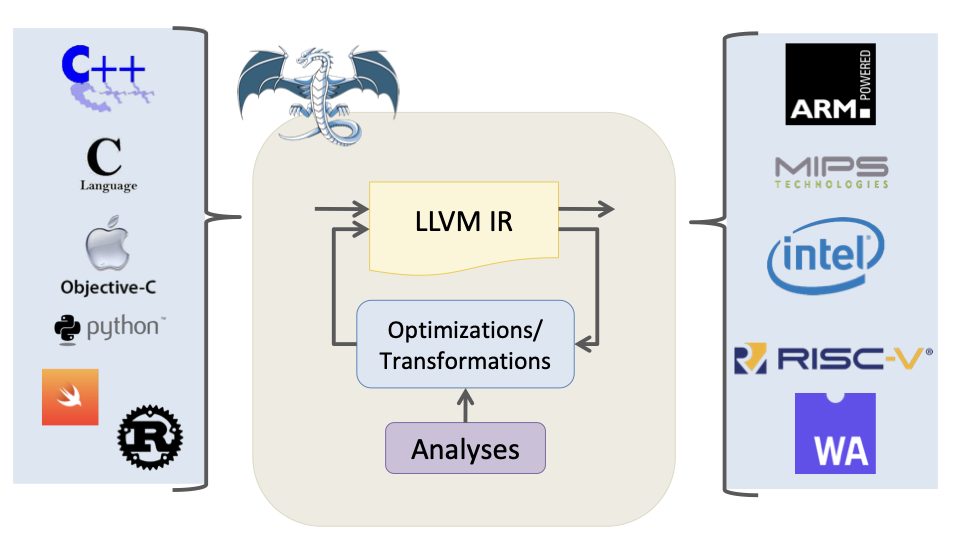
\includegraphics[scale=0.37]{thesis/llvm.png}
 
  \caption{LLVM compiler infrastrucutre with LLVM IR at its heart}
  \label{fig:your-label}
\end{figure}

LLVM IR is typed and in single static assignment form (SSA), which means that every variable has a type and is associated with only one specific definition point in the code. This allows for simplified compiler optimizations along def-use chains, as any use of a variable can be backtracked to a single place where the variable receives a value (def). 

[TO DO INSERT OVERVIEW OF LLVM IR ]

LLVM IR supports common types such as integers of different widths, as well as structured data. To handle non-initialized variables, LLVM IR supports an undef constant in its IR, which represents a set of possible values. When the LLVM compiler encounters an undef it is free to pick any convenient value of the correct type. Besides undef, LLVM IR  has poison values and undefined behaviour. All of these different notions of the future, where the compiler does not want to provide guarantees for a specific value or indicates a unsafe operation. This in turn makes the semantics of LLVM IR inherently non-deterministic and will be discussed in detail in section []. 

\textbf{RISC-V}
The target language of our to which LLVM IR will be lowered  is RISC-V, an open instruction set architecture developed at the University of Berkley. As the name suggests RISC-V is based on the reduced instruction set computer principle (RISC), where the ISA exhibits potentially many but simple instructions in comparison to CISC architectures.  RISC-V compromises an integer base ISA that comes with various added extensions allowing for a modular and domain-specific design of the ISA. RISC-V is available as a 32-bit (RV32) and 64-bit (RV64) architecture version while there are current efforts for  larger address space architectures like  RV128. 

The RISC-V base ISA specifies instructions for logic operations like integer manipulation, address calculation, control flow, and memory allowing for implementation of a simple general-purpose computer. Extensions like the bit manipulation extension (e.g ZBB)  supplement the base ISA and target code size reduction or performance improvement. The ZBB extension is defined for RV32 and RV64 (and follows the convention specified for RV64).
\section {Framework: Lean-MLIR(X)}
Lean-MLIR(X), which is part of the Lean-MLIR project, serves as the foundation for implementing our proposed instruction selection.
The Lean-MLIR project is an open-source framework for developing and reasoning about SSA-based compiler IRs within the Lean theorem prover. It enables users to formally verify compiler optimizations, particularly peephole rewrites. The framework is composed of several components that allow the representation of MLIR concepts in Lean, the verification of code transformations, and the creation of custom dialects. A dialect in Lean-MLIR mirros the concept of dialects in MLIR, hence a domain-specific IR.

Lean-MLIR provides a collection of pre-implemented dialects in Lean e.g LLVM IR dialect. To create a new dialect the user must specify syntax (types Ty and operations Op ) as well as the semantics for the dialect. This formalization of dialect definition within Lean allows for rigorous reasoning about the properties of the new dialect and the correctness of any transformations applied to it. Given a program written in a dialect using Lean-MLIR(X), the semantics of the program can be extracted using a denotation function. This allows to extract the meaning of computation and reason about the semantics of code. In this work we will modell a RISC-V dialect represent a ISA-like abstract ISA, which the can be mapped to machine code. Additionally, we use the LLVM IR dialect provided by Lean-MLIR project. [TO DO CHAPTRE REFERENCE ]
\begin{lstlisting}[language=Python, caption=LLVM IR dialect program in Lean based on the Lean-MLIR(X) framework]
 [llvm(w)| {
  ^bb0(%X : _, %Y : _):
    %v1 = llvm.sub %X, %X
    %r = llvm.xor %v1, %Y
    llvm.return %r
  }]
\end{lstlisting}
[TO DO EXAMPLE DIALECT AND HOW IT TRANSALTE TO COM AND VAR IN LEAN ]

Besides serving as a platform for defining and modeling MLIR style dialects in Lean, Lean-MLIR provides various components that are designed for verifying transformations applied to dialects.

The peephole rewriter tool applies user-specified rewrites to the representation of a program in a given dialect. A central feature of this tool is that it is proven to be semantics-preserving. Any rewrite applied by the tool is accompanied by a corresponding proof in Lean, ensuring that the transformation maintains the original meaning of the code, else Lean would not allow the user to apply the optimization as type checking would fail. 

In addition to the rewriter, the project includes a Dead Code Eliminator that performs verified dead code elimination. This optimization removes unreachable code and unused variable assignments. Like the rewriter, the dead code eliminator guarantees that transformations preserve program semantics. 
\begin{lstlisting}[language=Python, caption= DCE example]
 [llvm(w)| {
  ^bb0(%X : _, %Y : _):

  }]
\end{lstlisting}[TO DO DED CODE ELIMINATION EXAMPLE]

To make Lean-MLIR accessible to developers familiar with MLIR, the project provides an embedding of the MLIR abstract syntax tree and a parser built in Lean. This allows MLIR syntax to be written directly in Lean. Thanks to Lean’s metaprogramming capabilities, this syntax is parsed into an internal representation that supports formal verification—in Lean.

While Lean-MLIR offers a formally verified rewriter that focuses on rewrites within a single dialect and serves as a core foundation for this work, further extensions to the framework are needed to reason about transformations across dialects.  Part of this work will involve exploring cross-language/dialect transformations, which can be abstracted as rewrites across dialects. These extensions are necessary to implement our verified instruction selection that lowers between a source language and a target ISA. 








SO THE BACKGROUND STRUCTURE MIRRROS THE LOWERING PROCESS 
 LLVM IR
 MLIR 
 Lean-MLIR 
 Semantics of LLVM IR and 
 riscv 
 Sail semantics of RISCV/ Sail. 




\section {Semantics}
\subsection {LLVM IR semantics}
The Lean-MLIR project provides an implementation of MLIR's LLVM IR dialect in Lean. Given an LLVM IR program, one can leverage the MLIR toolchain—such as MLIR Transform—to lower the LLVM IR program into its MLIR representation.
The implementation of Lean-MLIR is designed so that these lowerings can be directly written in the Lean theorem prover, where they are parsed into an internal representation suitable for formal reasoning within Lean.
The semantics of the LLVM IR used in this project are defined by the Lean-MLIR project.

\subsection {RISC-V semantics}








